\chapter{Despliegue y pruebas}
\label{chap:despliegue}

\textcolor{red}{En este capítulo describiremos cómo se llevó a acabo el despliegue de la solución y las pruebas que se realizaron.}

\section{Despliegue}

Debido a la gran cantidad de microservicios que componen la solución, desde muy temprano fue necesario definir un plan de despliegue. Su número iba en aumento y era muy complicado gestionarlos a mano. Para ello, optamos entonces por empaquetarlos en contenedores de \texttt{Docker}\footnote{Página oficial: \url{https://www.docker.com/}}. Gracias a esto podíamos iniciarlos y pararlos fácilmente. Además que nos aporta una serie de ventajas interesantes: ejecución aislada de los procesos, gestión más fácil de las dependencias, entre otras. \cite{newmanBuildingMicroservicesDesigning2021,delatorreNETMicroservicesArchitecture2021}

\begin{wrapfigure}{r}{0.23\linewidth}
  \vspace{-25pt}
  \centering
  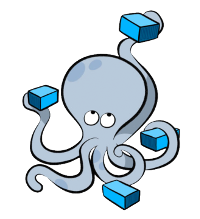
\includegraphics[scale=0.95]{cap_despliegue/images/docker-compose-logo}
  \vspace{-15pt}
\end{wrapfigure}

Para orquestar el despliegue de la solución optamos por \texttt{Docker Compose}\footnote{Página oficial: \url{https://docs.docker.com/compose/}}. Nos permite declarar la configuración del despliegue de nuestros servicios. Esto incluye los parámetros de ejecución, número de instancias, políticas de reinicio, etc. Aunque el bucle MAPE-K \foreign{english}{Lite} original corre sobre Kubernetes, no necesitábamos un orquestador tan ''pesado''. Nuestro plan era ejecutar la solución en un único \foreign{english}{host}.

\texttt{Docker Compose} también nos permite declarar las dependencias entre servicios. Esto fue clave para el despliegue del contenedor de \texttt{RabbitMQ}. Debido a que el protocolo requiere de una conexión permanente al bus\cite{johanssonPartRabbitMQBest2019}, todos los servicios que dependen de él deben desplegarse después. Por ello, declaramos una dependencia con este servicio y definimos una política de reintentos.

\subsection{Observabilidad y telemetría}

Un punto en el que queremos hacer hincapié es en la telemetría. Debido a que estamos tratando con un sistema distribuido, es complicado conocer su estado global en un momento determinado. Especialmente en este caso, en el que participan más de diez microservicios distintos. Si necesitáramos depurar y diagnosticar el comportamiento del sistema, es muy difícil trazar el impacto de una petición.

Por defecto, solo contábamos con los \emph{logs} (registros), que mostramos en la figura \ref{fig:console-logs}. Aparecen intercalados en una única ventana los de todos los servicios y peticiones concurrentes. Aunque nos pueden resultar utilidad, es una aproximación ineficiente. Incluyen demasiada información y es difícil de procesar para una persona. Además que, según aumente la carga de peticiones, aumentará el número de registros y se volverá más difícil de interpretar.

\begin{figure}[h]
  \centering
  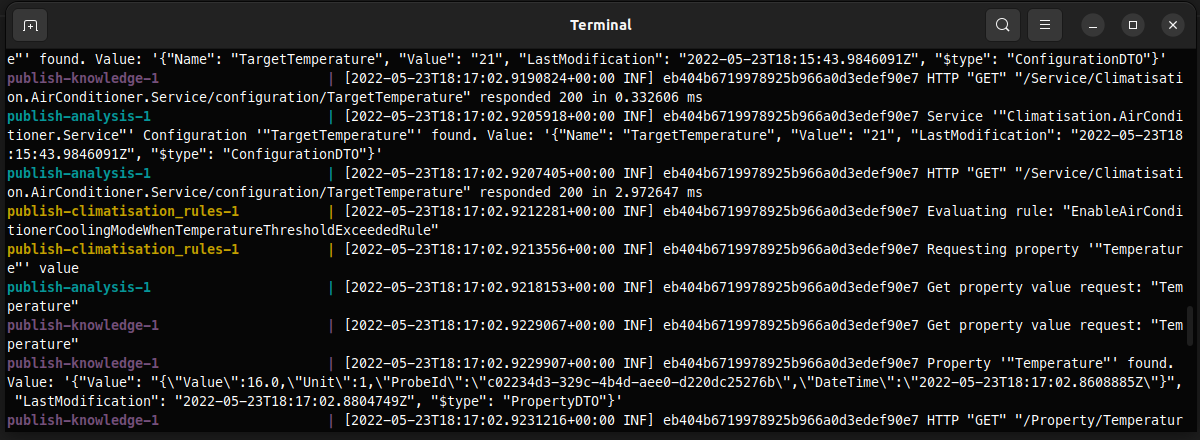
\includegraphics[scale=1.45]{cap_despliegue/images/console-logs}
  \caption{Extracto de \emph{logs} de una ejecución habitual.}
  \label{fig:console-logs}
\end{figure}

En el ámbito de los sistemas distribuidos requerimos de soluciones de monitorización y \foreign{english}{logging} más avanzadas. \cite{newmanBuildingMicroservicesDesigning2021} Nuestros servicios tendrán que recopilar y reportar datos de su funcionamiento, lo que se conoce como \textbf{telemetría}. Esto requerirá de \textbf{instrumentar} nuestros sistemas con distintas herramientas o \textbf{sondas}. Es exactamente lo mismo que hacemos en la etapa de monitorización del bucle MAPE-K.

Para explotar estos datos recurrimos a técnicas de \textbf{observabilidad}. Según \cite{parkerProblemDistributedTracing2020}, la observabilidad <<\emph{no es sólo un método para monitorizar sistemas en producción, si no también para ser capaces de entender su comportamiento usando un número relativamente bajo de señales}>>. Con \textbf{señales} se refiere a las distintas fuentes de información de telemetría de las que dispongamos.

La observabilidad nos ayuda a detectar variaciones en el funcionamiento de nuestro sistema. Estas puedes ser provocadas por errores, realentizaciones, etc. Hay un sinfin de causas. La observabilidad nos permite medirlas y explicar las causas de esta variación. en base a las señales. ayudarnos a: medir el impacto del funcionamiento de la aplicación sobre los usuarios y explicar la variación en esas medidades.


Existen tres tipos de señales que podemos capturar de nuestros servicios. Todas ellas son complementarias, ya que reflejan su funcionamiento desde distintas perspectivas. Son conocidos como \textbf{los tres pilares de la observabilidad}:

\begin{itemize}
  \item \textbf{Logs}: \textcolor{red}{A recording of an Event. Typically the record includes a timestamp indicating when the Event happened as well as other data that describes what happened, where it happened, etc. \cite{opentelemetryOpenTelemetryDocumentation2022} Provide extremely fine-grained detail on a given service, but have no built-in way to provide that detail in the context of a request. \cite{parkerProblemDistributedTracing2020}}

  \item \textbf{Métricas}: \textcolor{red}{Son agregados que nos permiten conocer el estado de las estancias de nuestros servicios. Records a data point, either raw measurements or predefined aggregation, as timeseries with Metadata. \cite{opentelemetryOpenTelemetryDocumentation2022}}

  \item \textbf{Trazas distribuidas}: \textcolor{red}{Tracks the progression of a single Request, called a Trace, as it is handled by Services that make up an Application. A Distributed Trace transverses process, network and security boundaries. \cite{opentelemetryOpenTelemetryDocumentation2022}  providing visibility into the operation of your microservice architecture. It allows you to gain critical insights into the performance and status of individual services as part of a chain of requests in a way that would be difficult or time-consuming to do otherwise. Distributed tracing gives you the ability to understand exactly what a particular, individual service is doing as part of the whole, enabling you to ask and answer questions about the performance of your services and your distributed system. \cite{parkerProblemDistributedTracing2020}}
\end{itemize}

Para poder capturar todos estos elementos, optamos por usar el estándar OpenTelemetry. Se trata de una librería estándar utilizada para instrumentar el código de las aplicaciones. Distintas compañías del ámbito de la telemetría software ofrecen APIs que capturan el output de esta librería.

Gracias a él pudimos capturar la telemetría de la siguiente forma implementar usando tres servicios distintos:

\begin{figure}[h]
  \centering
  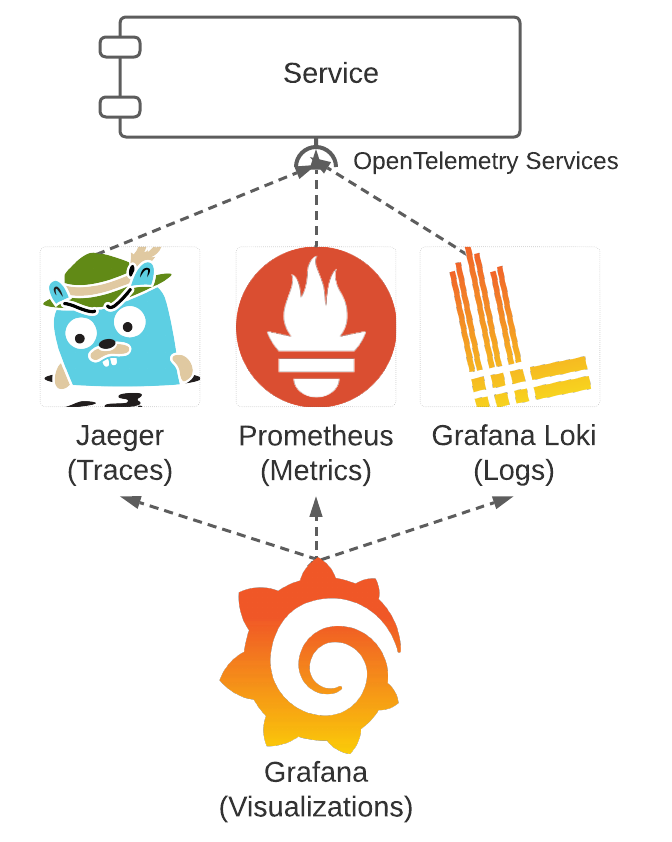
\includegraphics[scale=0.75]{cap_despliegue/images/observability-telemetry-collection}
  \caption{Extracto de \emph{logs} de una ejecución habitual.}
  \label{fig:observability-telemetry-collection}
\end{figure}

\subsubsection{Loki: Logs}
Lo primero que queremos ver es cómo mejorar nuestra estrategia de logging. Lo ideal es añadir identificadores de correlación (el traceID), que nos permita rastrear a través de los distintos servicios una misma traza. Por ejemplo, podemos filtrar a partir de ella para ver todos los detalles de los servicios que intervinieron.

\subsubsection{Jaeger: Trazas distribuidas}

Gracias a las trazas distribuidas, podemos ver todas las actividades por las que pasó una petición. En nuestro caso, podemos ver por todos los estados por los que paso.

\subsubsection{Prometheus: Métricas}


\subsubsection{Grafana: Visualización}

Desarrollamos un panel de monitorización con Grafana. Esto nos permitía consultar en un solo lugar las métricas, los logs y las trazas.

